% The "t" in documentclass vertically aligns the frame text to the top
% t-top c-center b-bottom 
\listfiles
\documentclass[croatian,t]{beamer} % must specify a language if using babel
\usetheme{CambridgeUS}
\usecolortheme{beaver}
\usepackage[utf8]{inputenc}
\usepackage{verbatim}
\usepackage{listings}
\usepackage[yyyymmdd,hhmmss]{datetime}
\usepackage{babel} % đ doesn't work without this package
% Changing of bullet foreground color not possible if {itemize item}[ball]
\DefineNamedColor{named}{BrickRed}{cmyk}{0,0.89,0.94,0.28}
\setbeamertemplate{itemize item}[triangle]
\setbeamercolor{title}{fg=BrickRed}
\setbeamercolor{itemize item}{fg=BrickRed}
\setbeamercolor{section number projected}{bg=BrickRed,fg=white}
\setbeamercolor{subsection number projected}{bg=BrickRed}
% Beamer defines "\Tiny" so we have to redefine it to "\tiny"
\let\Tiny=\tiny
\renewcommand{\dateseparator}{.}
\newcommand{\todayiso}{\twodigit\day \dateseparator \twodigit\month \dateseparator \the\year}
\title[NKOSL]{Napredno korištenje operacijskog sustava Linux}
\subtitle{Sklopovlje i arhitektura}
\author{Goran Cetušić}
\author[Goran Cetušić]{Goran Cetušić\\{\small Nositelj: dr. sc. Stjepan Groš}}
\institute[FER]{Sveučilište u Zagrebu \\
				Fakultet elektrotehnike i računarstva}
\date{\todayiso}

\begin{document}
    %\beamerdefaultoverlayspecification{<+->}
    {
    \setbeamertemplate{headline}[] % still there but empty
    \setbeamertemplate{footline}{}
    \begin{frame}
        \maketitle
    \end{frame}
    }
    
    \begin{frame}
        \tableofcontents
    \end{frame}
    
    \section{Pokretanje računala}
    \begin{frame}{CPU}
    	\begin{itemize}
    		\item Prva instrukcija koju procesor izvrši nalazi se na dobro poznatoj memorijskoj adresi
    		\begin{itemize}
    			\item Na tu memorijsku lokaciju vezan je čip koji sadrži \emph{firmware}
    			\item \emph{firmware} je prvi kod koji se počne izvršavati pri pokretanju računala
    		\end{itemize}
    		\item \emph{firmware} na matičnoj ploči je \emph{flash} čip koji je moguće reprogramirati
    		\begin{itemize}
    			\item Čip je obično lako zamijeniti korištenjem posebnih kliješta
    			\item Moguće je postojeće naredbe zamijeniti vlastitima
    		\end{itemize}
    		\item Postoje stotine vrsta \emph{flash} (EEPROM) čipova koji dolaze u različitim kućištima sa različitim performansama i namjenama
    		\item \emph{firmware} tipično dolazi sa PLCC32 čipovima koji su izravno zalemljeni na matičnu ploču ili se nalaze u utorima koji su zalemljeni na ploču
    	\end{itemize}
    \end{frame}
    
    \begin{frame}{EEPROM}
    	\begin{columns}
    		\begin{column}{4cm}
    			\begin{figure}
					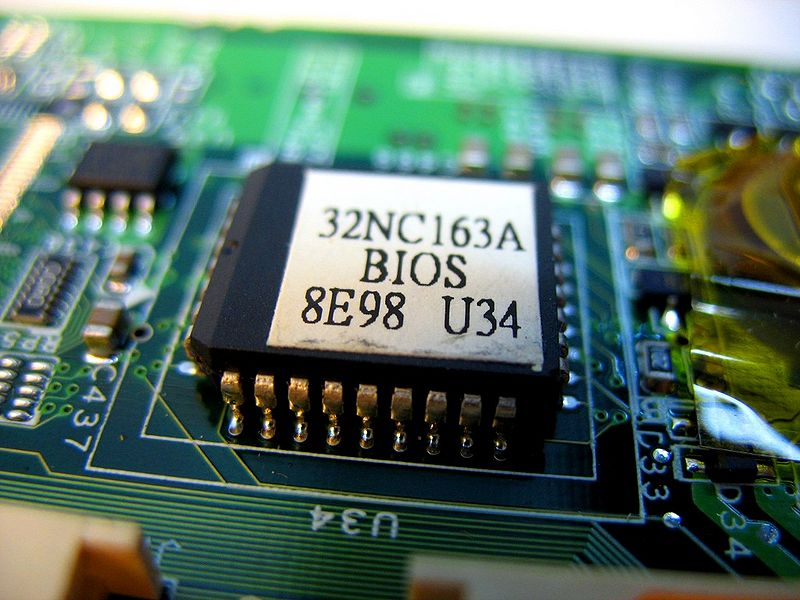
\includegraphics[width=0.62\textwidth]{../pics/800px-Soldered_plcc32.jpg}
					\caption{Zalemljeni PLCC32}
				\end{figure}
				\begin{figure}
					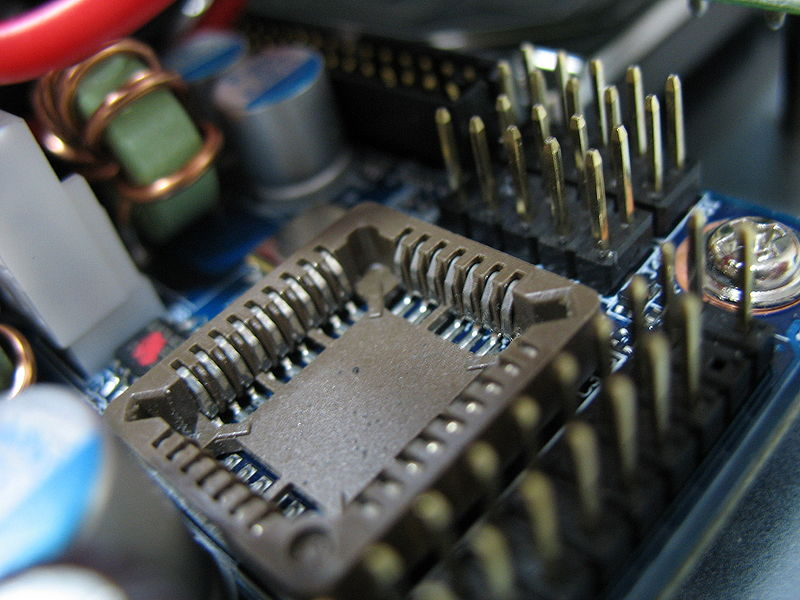
\includegraphics[width=0.62\textwidth]{../pics/800px-Empty_plcc32_socket.jpg}
					\caption{PLCC32 socket}
				\end{figure}
			\end{column}
			\begin{column}{4cm}
				\begin{figure}
					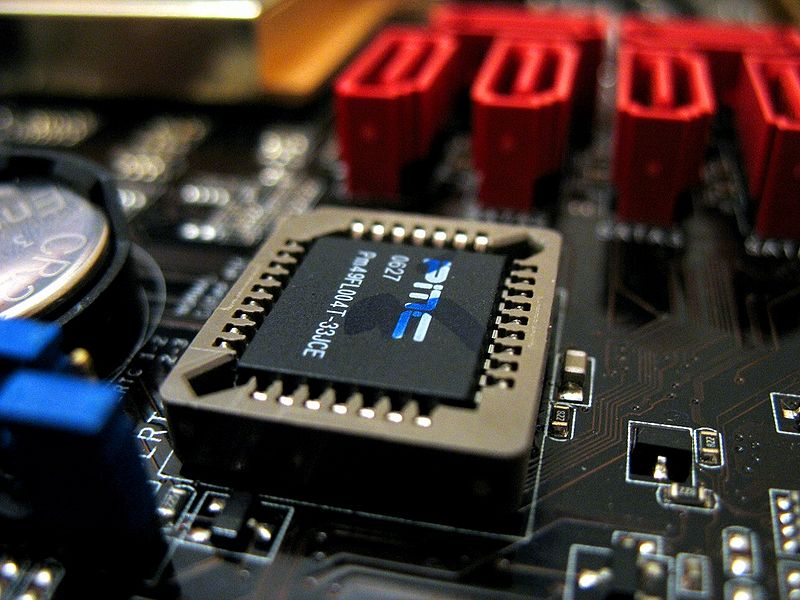
\includegraphics[width=0.62\textwidth]{../pics/800px-Plcc32_in_socket.jpg}
					\caption{PLCC32 u socketu}
				\end{figure}
				\begin{figure}
					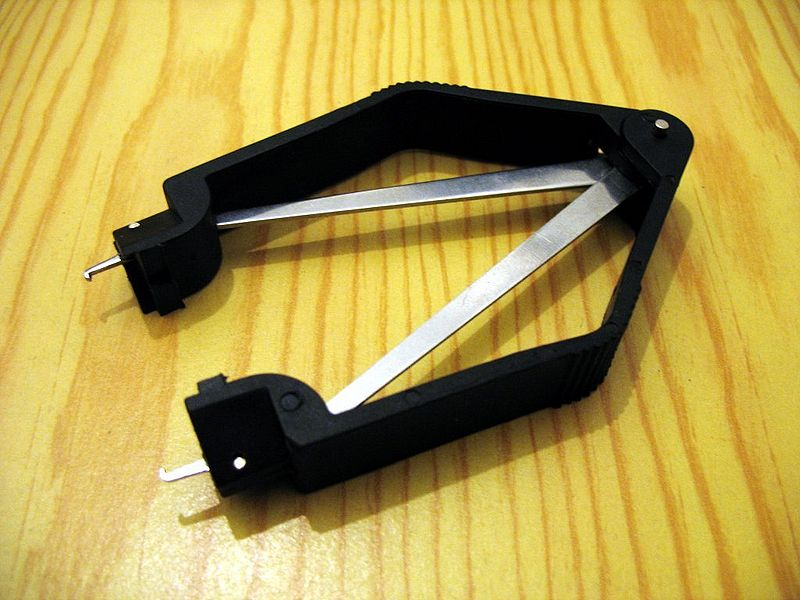
\includegraphics[width=0.62\textwidth]{../pics/800px-Plcc_tool.jpg}
					\caption{PLCC kliješta}
				\end{figure}
			\end{column}
			\begin{column}{4cm}
				\begin{figure}
					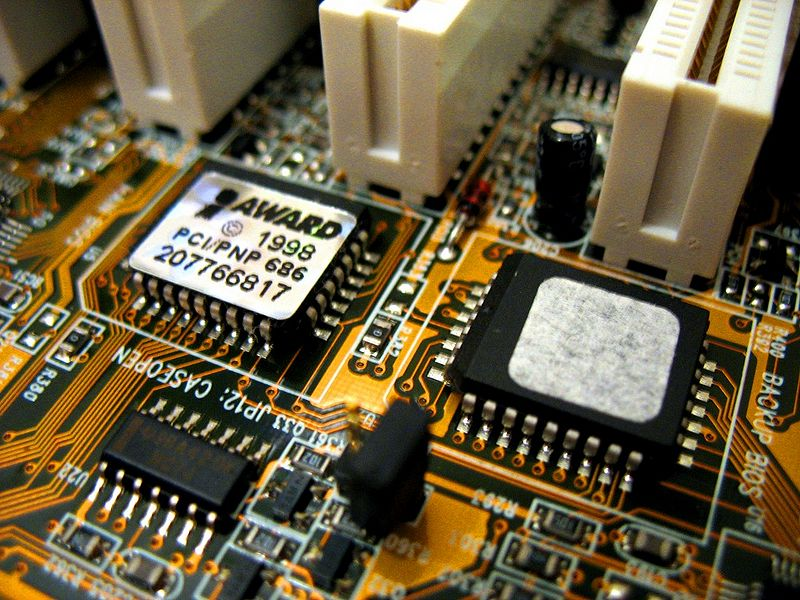
\includegraphics[width=0.62\textwidth]{../pics/800px-Dual_plcc32_soldered.jpg}
					\caption{Dual BIOS}
				\end{figure}
				\begin{figure}
					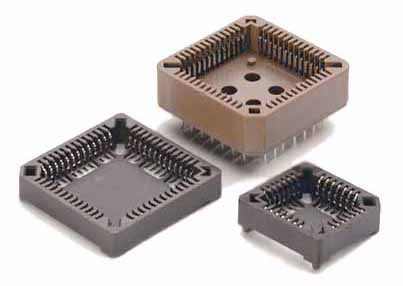
\includegraphics[width=0.62\textwidth]{../pics/plcc_socket.jpg}
					\caption{PLCC socket}
				\end{figure}
			\end{column}
		\end{columns}
    \end{frame}

    \begin{frame}
		\begin{figure}
			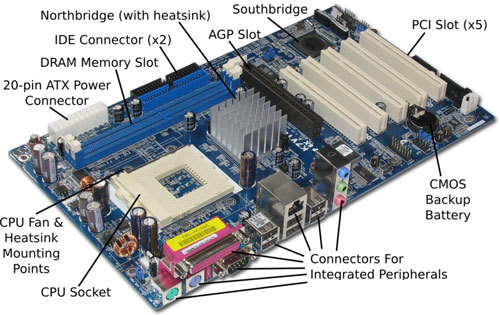
\includegraphics[width=0.7\textwidth]{../pics/motherboard-parts.jpg}
			\caption{Matična ploča}
		\end{figure}
    \end{frame}    

    \begin{frame}
		\begin{figure}
			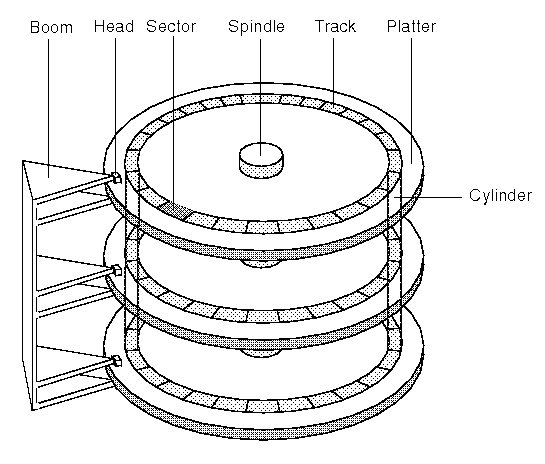
\includegraphics[width=0.7\textwidth]{../pics/harddisk.jpg}
			\caption{Tvrdi disk}
		\end{figure}
    \end{frame}    
    
    \begin{frame}
    	\begin{columns}[c]
    		\begin{column}{4cm}
    			\begin{figure}
					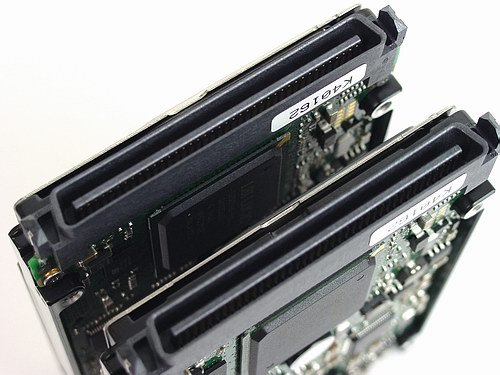
\includegraphics[width=0.62\textwidth]{../pics/scsi_disk.jpg}
					\caption{SCSI disk}
				\end{figure}
			\end{column}
			\begin{column}{4cm}
				\begin{figure}
					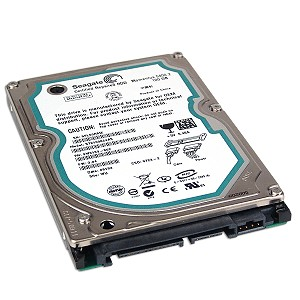
\includegraphics[width=0.62\textwidth]{../pics/sata_disk.jpg}
					\caption{SATA disk}
				\end{figure}
   				\begin{figure}
					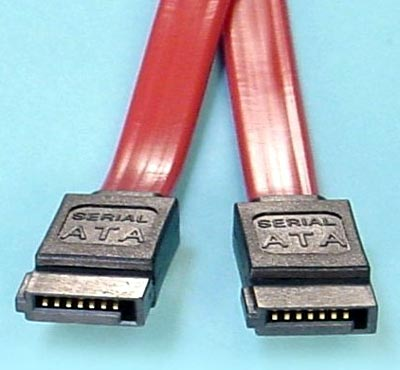
\includegraphics[width=0.62\textwidth]{../pics/sata_connector.jpg}
					\caption{SATA konektor}
				\end{figure}
			\end{column}
			\begin{column}{4cm}
				\begin{figure}
					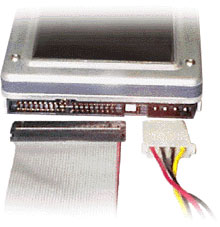
\includegraphics[width=0.62\textwidth]{../pics/pata_disk.jpg}
					\caption{PATA disk}
				\end{figure}
   				\begin{figure}
					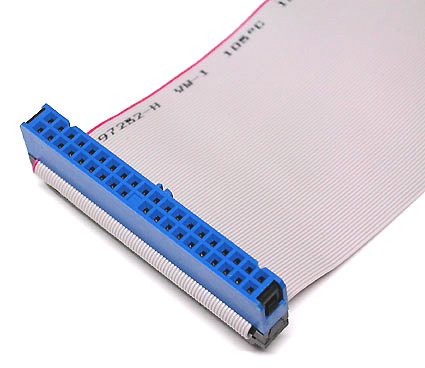
\includegraphics[width=0.62\textwidth]{../pics/pata_connector.jpg}
					\caption{PATA konektor}
				\end{figure}
			\end{column}
		\end{columns}
    \end{frame}
    
    \section{BIOS+MBR}
    \begin{frame}{BIOS (Basic Input / Output System)}
    	\begin{itemize}
    		\item Uloga BIOS-a se mijenjala tijekom godina
    		\begin{itemize}
    			\item Nekada se korištenjem njegovog API-a pristupalo uređajima
    			\item Danas primarno služi za pokretanje operacijskog sustava
    		\end{itemize}
    		\item Postoje novije i modernije implementacije
    			\begin{itemize}
    				\item EFI, Coreboot, OpenBIOS...
    				\item BIOS razvija samo nekoliko komerijalnih tvrtki
    			\end{itemize}
    		\item Moguće je (oprezno) zamijeniti BIOS npr. Corebootom
    			\begin{itemize}
    				\item Može doći do greške tijekom \emph{flashanja} čipa i računalo neće moći podići operacijski sustav
    				\item Budući da se obično taj postupak radi iz OS-a, jedini način kako riješiti problem je stavljanje drugog čipa koji sadrži funkcionalan BIOS
    				\item Iz tog razloga neke matične ploče imaju Dual BIOS - dva čipa sa zasebnim BIOS-om gdje je svaki u stanju podići OS
    			\end{itemize}
    		\begin{itemize}
    			\item MS-DOS koristi BIOS za pristupanje uređajima
    		\end{itemize}
    	\end{itemize}
    \end{frame}
    
    \begin{frame}{POST (Power On Self Test)}
    	\emph{"The task of BIOS is just load the OS and get the hell out of there"}
    	\begin{itemize}
    		\item BIOS ima nekoliko zadaća prije nego preda upravljanje OS-u
    		\item POST je dijagnostički program u BIOS-u koji provjerava prisustvo RAM-a i komponenti na matičnoj ploči
    		\begin{itemize}
    			\item Ako u ovom stadiju dođe do greške, BIOS kombinacijom  kratkih i dugih zvučnih signala dojavi korisniku što je uzrok greške
    			\item Značenje signala ovisi o proizvođaču BIOS-a i najčešće se može pronaći u priručniku proizvođača
    		\end{itemize}
    		\item Ako sve prođe dobro i BIOS uspije pronaći video karticu, ispisuje status na monitor
			\item BIOS u CMOS memoriju na matičnoj ploči sprema postavke poput datuma, redoslijeda pretraživanja uređaja, ili lozinku za postavke
			\begin{itemize}
			\item Budući da CMOS za spremanje podatak zahtijeva stalan izvor napona, koristi se mala baterija za napajanje kada je računalo ugašeno
			\item Vađenjem baterije postavke su poništene		
			\end{itemize}
    	\end{itemize}
    \end{frame}
    
	\begin{frame}{ATA/SCSI}
		\begin{itemize}
			\item \emph{firmware} operacijski sustav uglavnom podiže sa diskova
			\item Najpopularnija sučelja za komunikaciju sa diskovima su		
			\begin{itemize}
				\item SCSI - Small Computer System Interface
			\end{itemize}
			\begin{itemize}
				\item ATA - Advanced Technology Attachment
				\begin{itemize}
					\item IDE/PATA - Parallel Advanced Technology Attachment
					\item SATA - Serial Advanced Technology Attachment				
				\end{itemize}
			\end{itemize}
			\item BIOS koristi INT13h sučelje za pristupanje diskovima
				\begin{itemize}
					\item Međutim, maksimalna veličina diska je 528MB (CHS)
					\item Premalo za današnje diskove
				\end{itemize}
			\item Budući da se BIOS i dalje koristi, adrese se prevode
			\item Primjer LHS prijevoda \\
			~~~~~LBAsector = ((Cyl * DiskHeads) + Head) * DiskSectors + Sec - 1
			\item Poanta: BIOS je nužno zlo
		\end{itemize}
	\end{frame} 

	\begin{frame}{MBR (Master boot record)}
    \begin{columns}[c]
    % It's necesarry to give the column size
        \begin{column}{7cm}
            \begin{itemize}
            \item Na prvih 512 bajta diska nalazi se MBR
            \item BIOS kao zadnju akciju pokrene kod na prvih 446 bajta diska
            \item 64 bajta u MBR-u rezervirano je za informacije o particijama
            \begin{itemize}
            	\item 16B za svaku particiju
            	\item Max. broj primarnih particija je 4
            \end{itemize}
            \item Magic number je obično 0xAA55
            \begin{itemize}
            	\item BIOS po ovom broju prepoznaje da može pokrenuti sustav sa diska
            	\item Po rasporedu u CMOS-u određuje koji će biti prvi uređaj
            \end{itemize}
            \end{itemize}
        \end{column}
        \begin{column}{5cm}
            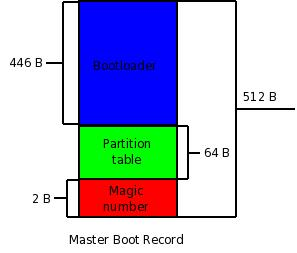
\includegraphics[scale=0.5]{../pics/mbr.jpg}
        \end{column}
    \end{columns}
	\end{frame}
	
	\begin{frame}{EBR (Extended boot record)}
		\begin{itemize}
            \item Jedna particija može biti \emph{extended}
            \begin{itemize}
            	\item Takva proširena particija ima EBR
            	\item EBR se nalazi unutar 16 bajta u MBR-u na mjestu zapisa o particiji
            \end{itemize}
            \item Jedna logička particija pokazuje na sljedeću itd.
		\end{itemize}
		\begin{center}
			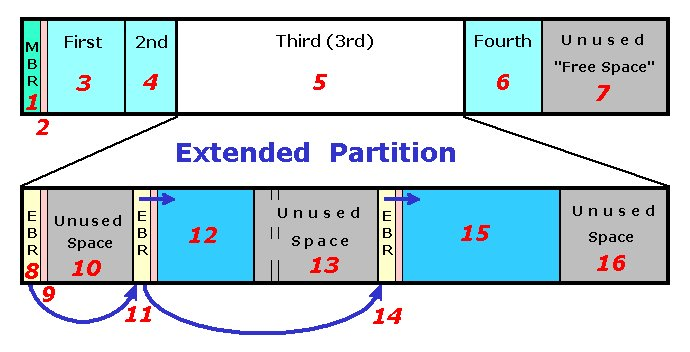
\includegraphics[width=0.7\textwidth]{../pics/EBRreality.jpg}		
		\end{center}
	\end{frame}

    \begin{frame}
		\begin{figure}
			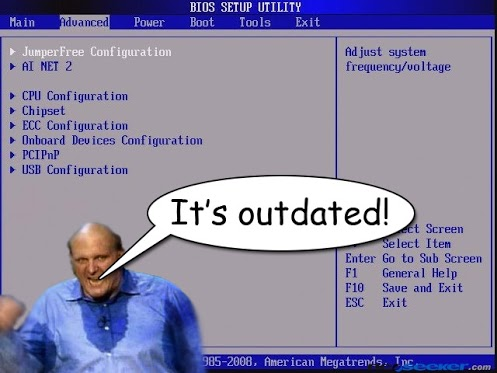
\includegraphics[width=0.7\textwidth]{../pics/bios-outdated-uefi.jpg}
		\end{figure}
    \end{frame}  
	
	\section{UEFI+GPT}
    \begin{frame}{UEFI (Unified Extensible Firmware Interface)}
    	\begin{itemize}
    		\item Moderna zamjena za BIOS
    		\begin{itemize}
    			\item Ne izvršava slijepo kod na disku kao BIOS
    		\end{itemize}
    		\item Nakon pokretanja sustava:
    			\begin{enumerate}
    				\item POST
    				\item \emph{firmware} je učitan (UEFI)
    				\item UEFI utvrđuje lokaciju sljedeće aplikacije (disk i particiju)
    				\item UEFI pokreće aplikaciju
    				\item aplikacija preuzima podizanje sustava
    			\end{enumerate}
    		\item Proizvođači prelaze na EFI standard (Extensible Firmware Interface)
    		\item Međutim, zbog kompatibilnosti je prijelaz spor
    	\end{itemize}
    \end{frame}
    
	\begin{frame}[fragile] % fragile is needed for listings in beamer
	\frametitle{EFI particija}
		\begin{itemize}
		\item EFI se nalazi na posebnoj particiji
			\begin{itemize}
				\item FAT12, FAT16 ili FAT32
			\end{itemize}
		\begin{lstlisting}[basicstyle={\tiny\ttfamily},language=bash]
# parted /dev/sda print
Model: ATA HITACHI HTS72323 (scsi)
Disk /dev/sda: 320GB
Sector size (logical/physical): 512B/512B
Partition Table: gpt
Disk Flags: 

Number  Start   End    Size   File system  Name                  Flags
 1      1049kB  211MB  210MB  fat16        EFI System Partition  boot
 2      211MB   735MB  524MB  ext4
 3      735MB   288GB  287GB   
 		\end{lstlisting}
		\end{itemize}
	\end{frame}
    
	\begin{frame}{GPT (GUID partition table)}
    \begin{columns}[c]
    % It's necesarry to give the column size
        \begin{column}{7cm}
            \begin{itemize}
            \item Protective MBR
            \begin{itemize}
            	\item 64KB s jednom primarnom particijom
            \end{itemize}
            \item Primary GPT header
            \begin{itemize}
            	\item Sadrži GUID diska, lokaciju primarne GPT tablice i sekundarnog zaglavlja itd.
            \end{itemize}
            \item Primary GPT table
            \begin{itemize}
            	\item Popis particija s njihovim GUID-ovima
            \end{itemize}
			\item Secondary GPT table
			\begin{itemize}
				\item Kopija primarne tablice, služi za oporavak
			\end{itemize}
			\item Secondary GPT header
			\begin{itemize}
				\item Sadrži lokaciju sekundarne tablice i primarnog zaglavlja
			\end{itemize}
            \end{itemize}
        \end{column}
        \begin{column}{5cm}
            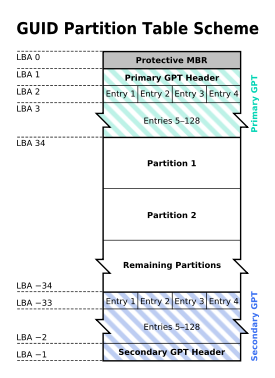
\includegraphics[scale=0.5]{../pics/gpt.png}
        \end{column}
    \end{columns}
	\end{frame}
	
	\section{Informacije o uređajima}
	\begin{frame}{Sustav}
		\begin{itemize}
			\item Informacije o sustavu nalaze se u /proc
			\item Za sklopovlje:
		\begin{verbatim}
			\tiny
			/proc/acpi        * Power Management  \\
			/proc/bus/pci     * Note: on some distributions this may be /proc/pci \\
			/proc/cpuinfo     * processor information \\
			/proc/dma \\
			/proc/interrupts \\
			/proc/iomem \\
			/proc/ioports \\
			/proc/irq \\
			/proc/meminfo \\
			/proc/uptime      * Since when the system is up and running. \\
			/proc/sys/kernel  * Kernel information.\\
			/proc/sys/net     * Network information.\\
			/proc/partitions  * Hard drive partitions information.\\
			/proc/scsi        * SCSI information.\\
			/proc/mount       * Mounted file system information.\\
			/proc/devices     * List the loaded drivers.\\
			/proc/bus         * Bus information. \\
			/proc/version     * Linux version.\\
		\end{verbatim}
			\item Zadatak: pregledati sadržaj svih datoteka i ustanoviti čemu služe
		\end{itemize}
	\end{frame}
	
	\begin{frame}[fragile] % fragile is needed for listings in beamer
	\frametitle{Diskovi}
		\begin{itemize}
		\item Alati za dobavljanje informacija o diskovima su:
			\begin{itemize}
				\item \textbf{hdparm} - za ATA sučelja
				\item \textbf{sdparm} - za SCSI sučelja
			\end{itemize}
		\begin{lstlisting}[basicstyle={\tiny\ttfamily},language=bash]
hdparm -v /dev/sda

/dev/sda:
 multcount     = 16 (on)
 IO_support    =  0 (default) 
 readonly      =  0 (off)
 readahead     = 256 (on)
 geometry      = 7296/255/63, sectors = 117210240, start = 0
		\end{lstlisting}
		\begin{lstlisting}[basicstyle={\tiny\ttfamily},language=bash]
hdparm [options] [devices]
Common options:
-g: Get the disk geometry.
-C: Display the power mode of the hard drive.
 active/idle: Normal operation,
 Standby: Low  power  mode,
 or sleeping: Lowest power mode.
-v: Display  all  settings,  except  -i
 This is also the default behaviour when no flags are specified.
 		\end{lstlisting}
		\end{itemize}
	\end{frame}
	
	\begin{frame}[fragile]
	\frametitle{PCI sabirnica}
		\begin{itemize}
			\item Prvo je potrebno razjasniti: Linux multifunkcionalne uređaje poput zvučnih kartica tretira zasebno po funkcijama*
			\item Najčešće se periferne jedinice poput mrežnih kartica spajaju na PCI sabirnicu
			\item lspci nareba ispisuje PCI uređaje na sabirnici
				\begin{itemize} 
					\item Korisna je za detektiranje uređaja na računalu
					\item Podrška Linux-a za specifične uređaje provjerava se lspci ispisom 
				\end{itemize}
			\item Ispis je oblika: 00:1c.3 0604: 8086:27d6 \\
1. 00 – identifikator sabirnice \\
2. 1c – identifikator uređaja na sabirnici \\
3. 3 – funkcija* \\
4. 0604 – tip uređaja \\ 
5. 8086:27d6 – proizvođač i identifikator uređaja \\
		\end{itemize}
	\end{frame}
	
	\begin{frame}[fragile]
	\frametitle{USB}
		\begin{itemize}
			\item Naredba \textbf{lsusb} ispisuje podatke o USB uređajima
			\item /proc/bus/usb pokazuje informacije o USB uređaju
			\begin{lstlisting}[basicstyle={\tiny\ttfamily},language=bash]
# lsusb
Bus 001 Device 001: ID 1d6b:0002  
Bus 005 Device 001: ID 1d6b:0001  
Bus 004 Device 001: ID 1d6b:0001  
Bus 003 Device 002: ID 04b0:012e Nikon Corp. Coolpix 5600 (ptp)
Bus 003 Device 001: ID 1d6b:0001  
Bus 002 Device 001: ID 1d6b:0001
			\end{lstlisting}
			\item Moderne distribucije imaju /sys direktorij sa strukturiranim informacijama o uređajima \\
				/sys/bus/usb \\
				/sys/bus/pci \\
			\item Identifikatori proizvođača za USB i PCI uređaje nalaze se u datotekama /usr/share/hwdata/pci.ids i /usr/share/hwdata/usb.ids
		\end{itemize}
	\end{frame}
	
	\begin{frame}{Ostale naredbe}
		\begin{itemize}
			\item Zadatak: proći kroz sve navedene naredbe i ispitati funkcije
		\begin{itemize}
			\item dmesg
			\item free
			\item uptime
			\item uname
			\item vmstat
			\item top i htop
			\item df
			\item du
			\item hostname
			\item fuser
			\item lsof
		\end{itemize}
		\end{itemize}
	\end{frame}
	
	\section{Zadaci}
	\begin{frame}
		\begin{enumerate}
		\item Kolika je veličina radne memorije na sustavu?
		\item Pomoću lspci prikažite PCI sustav u obliku stabla.
		\item Koliko PCI sabirnica postoji na sustavu?
		\item Kako pomoću lspci ispisati samo Intelove uređaje?	
		\item Kako postaviti IDE disk da radi samo u read-only modu?
		\item Pomoću uname naredbe ispisati samo tip procesora.
		\item Koliko dugo je sustav podignut?
		\item Koji procesi pristupaju /home direktoriju?
		\item Ispisati zauzeće particija u megabajtima.
		\item Ispisati sve IPv4 konekcije.
		\item Naredbom flashrom pročitati BIOS.
		\end{enumerate}
	\end{frame}	
	
	\section{}
	\begin{frame}{Literatura}
		\begin{tiny}
			\url{https://wiki.archlinux.org/index.php/Unified_Extensible_Firmware_Interface} \\
			\url{https://wiki.archlinux.org/index.php/GUID_Partition_Table} \\
			\url{http://www.pcguide.com/ref/mbsys/bios/boot.htm}
			\url{http://www.bit-tech.net/hardware/storage/2010/06/01/are-we-ready-for-3tb-hard-disks/2}	\url{http://en.wikibooks.org/wiki/LPI_Linux_Certification/Configure_Fundamental_BIOS_Settings}
			\url{http://www.centos.org/docs/5/html/5.1/Deployment_Guide/s1-proc-topfiles.html}
			\url{http://prefetch.net/articles/linuxpci.html}
			\url{http://mirror.href.com/thestarman/asm/mbr/PartTables.htm}
			\url{http://pciids.sourceforge.net/}
			\url{http://prefetch.net/articles/linuxpci.html}
		\end{tiny}
	\end{frame}
\end{document}
